\section{Implementace}
Meteostanice je implementována pomocí 2 \textit{RTOS tasků} -
task pro aktualizaci hodnot vlhkosti, teploty a aktualizace displeje
a task pro změnu \textit{flagu} obsahu displeje.

Každých 5 sekund je provedena aktualizace flagu pro obsah displeje.
Na základě tohoto flagu je při aktualizaci hodnot zobrazena informace
o teplotě nebo vlhkosti. Tato aktualizace probíhá každé 3 sekundy.
Při zobrazení těchto informací je na displeji zobrazena číselná hodnota,
text informující o způsobu reprezentace
této číselné hodnoty (teplota/vlhkost) a ikona plnící stejnou funkčnost
jako text (kapka - reprezentující vlhkost / teploměr - reprezentující teplotu).

\begin{figure}[h]
	\centering
	\begin{subfigure}[h!]{0.4\textwidth}
		\centering
		
\includegraphics[width=0.3\textwidth]{penis.png}
		\caption{Ikona teploměru}
	\end{subfigure}
	\hfill
	\begin{subfigure}[h!]{0.4\textwidth}
		\centering
		
\includegraphics[width=0.3\textwidth]{humidity.png}
		\caption{Ikona vlhkosti}
	\end{subfigure}
\end{figure}

\subsection{Senzor}
Se senzorem je možné komunikovat pomocí 2 módů
- \textbf{\textit{Single shot}} a \textbf{\textit{Periodic}}.
Zamýšlené použití \textit{single shot} módu je získání
informaci o teplotě/vlhkosti v nepriodických intervalech
nebo v intervalech s velkou šířkou (větší než 0.5 sekund). \textit{Periodic} mód
je použit v přesně opačném případě, kdy perioda je menší než 0.5 sekund
(největší jednotka meření za sekundu).

Při implementaci byl zvolen \textit{single shot} mód s periodou 1 sekundy.
S takovou malou periodou je možné zvolit i periodický mód.
Pokud bychom však takovou meteostanici chtěli někde reálně použít,
tak by bylo vhodné (dle případu užití) zvolit větší periodu,
aby mezi jednotlivými měřeními mohl být senzor v režimu spánku
pro snížení spotřeby energie. Perioda o velikosti 1 sekundy byla
tedy zvolena primárně pro demonstrační účely.

Použití senzoru v single shot módu je možné shrnout do 3 kroků:
\begin{enumerate}
	\item Zaslání příkazu (I2C write header a data 0x2400)
	\item Vyčkání na dokončení měření
	\item Přečtení dat (I2C read header)
\end{enumerate}

\begin{figure}[h!]
	\centering
	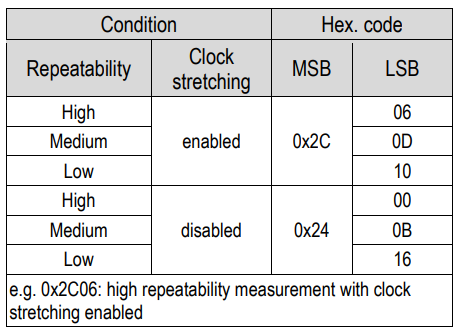
\includegraphics[width=0.5\textwidth]{sht3x_init.png}
	\caption{Příkazy pro získání informací ze senzoru pro single shot mód. \cite{sht3x-doc}}
\end{figure}

\newpage

Na obrázku výše je možné vidět, že je možné nastavit 2 parametry:
\begin{itemize}
	\item Clock stretching, který obecně slouží pro zpomalení (- dočasné zastavení) SCL signálu slave zařízením
	(senzorem v tomto případě) v případě, že toto zařízení právě vykonává nějakou činnost
	(probíhá měření). Zvolen "disabled".
	\item Repeatability, který určuje, jak dlouho bude probíhat měření.
	Maximální doba měření je 2.5ms (low), 6.5ms (medium) a 15.5ms (high).
	Delší měření jsou přesnější, avšak mají větší spotřebu.
	Zvolen "high".
\end{itemize}

Senzor je možné provozovat pouze v pracovních teplotách 5°C - 60°C.
Dle datasheetu SHT3x \cite{sht3x-doc} může vystavení senzoru mimo
pracovní teplotu způsobit odchylku od reálných hodnot.
Dlouhodobé vystavení těmto podmínkám může uskutečnit tuto odchylku permanentní.
